\section{Data Preprocessing}

\begin{figure}[ht]
    \centering
    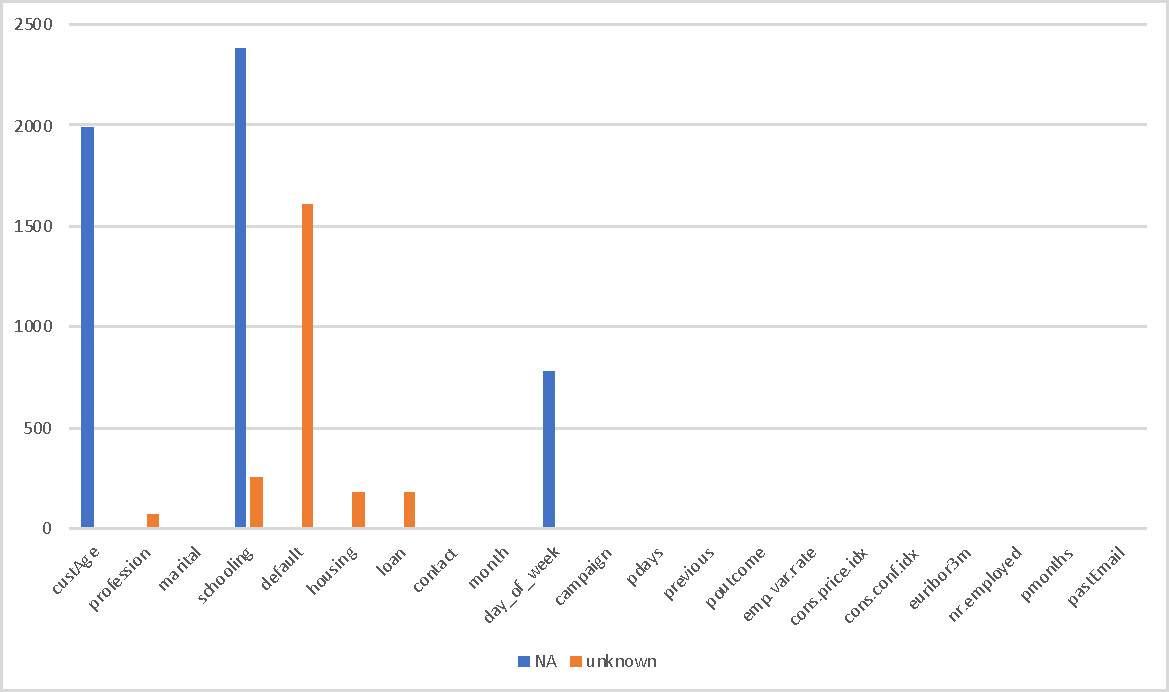
\includegraphics[width=0.5\textwidth]{img/missing.pdf}
    \caption{missing dat distirbution}
    \label{missing}
\end{figure}

\subsection{Fill missing values}
We find there are many missing values in training set, like `NA', `unknown'. we think that just remove these samples whose feature includes missing value is not a good idea because there are almost 30\% data include missing value.

Actually, most of the missing values are in `custAge', `schooling', `default' and `day\_of\_week' (details have been shown in Fig.\ref{missing}), a basic idea is fill these values with 0 or random sample some value from this attribute, but it will bring many noise data, so we deicde to select nearest sample which has real value to fill in.

\subsection{Normalization}
There are 4 type of feature: \textbf{bool}, \textbf{int}, \textbf{float} and \textbf{enum}. For int and float type, different feature has big difference of scale and region, so we should do normalization. a common normalization algorithm is \textbf{z-score}:
\begin{align*}
    z = \frac{z - \mu}{\sigma}
\end{align*}
where $\mu$ is the mean of population, $\sigma$ is the standard deviation of the population.



On the other hand, we use \textbf{one-hot code} to handle bool and enum type: if an enum feature has 4 different attribute, we will encode it into a 4 dimension vector, and each dimension correspond to an attribute.


\subsection{Feature Selection}
There are many attributes in oen sample feature, which will cause the curse of dimensionality, which means that will let model complex and hard to train, so feature selection is important.



In Fig.\ref{cor}, obviously there are some features are linearly dependent, which isn't important and should be removed. 

\subsection{Handling unbalanced data}
The final target of us is train a model to predict customer who brings profits(larger than 30). but these people are only 10\% of total train set, i.e. wanted people is too little to train a robust model, so we should create some new data to balance.

\begin{figure}[ht]
    \centering
    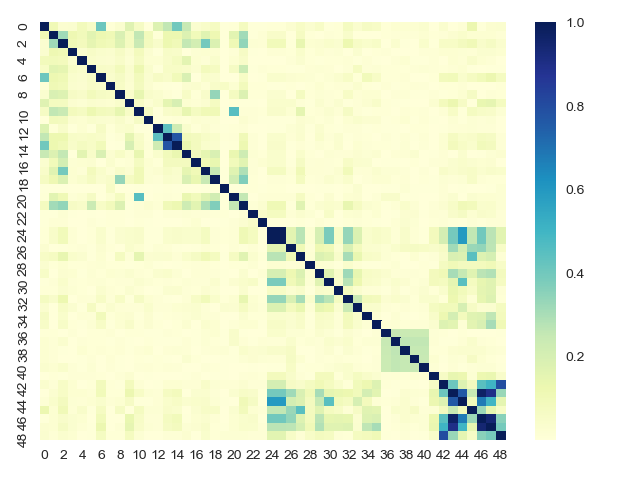
\includegraphics[width=0.5\textwidth]{img/Cor.png}
    \caption{Corelation Matirx}
    \label{cor}
\end{figure}

\begin{figure}[ht]
    \centering
  \subfloat[origin]{%
       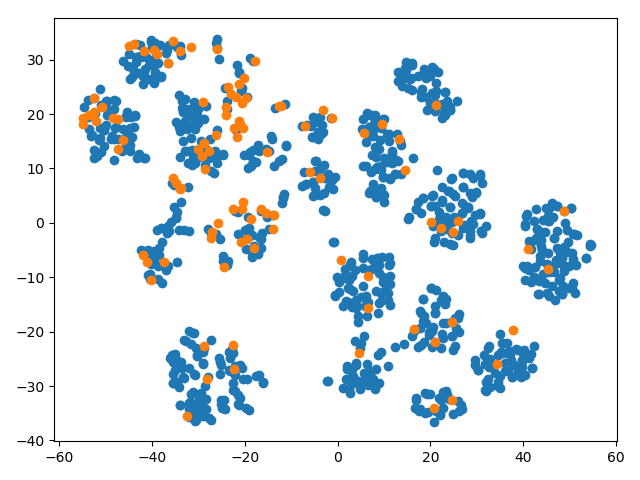
\includegraphics[width=0.45\textwidth]{img/unbalanced.png}}
    \label{1a}
  \subfloat[oversampling]{%
        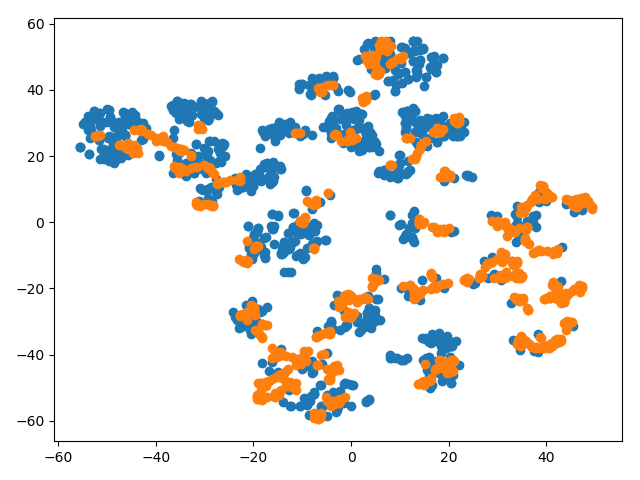
\includegraphics[width=0.45\textwidth]{img/balanced.png}}
    \label{1b}
  \caption{oversampling}
  \label{oversampling} 
  \end{figure}


\textbf{SMOTE}(Synthetic Minority Oversampling Technique) is a well known oversampling method to handle unbalanced data.